% !TeX TXS-program:compile = txs:///pdflatex/[--shell-escape]
\documentclass[landscape,a4paper]{article}
\usepackage[table]{xcolor}
\usepackage[normalem]{ulem}
\usepackage{tikz}
\usetikzlibrary{shapes,positioning,arrows,fit,calc,graphs,graphs.standard}
\usepackage[nosf]{kpfonts}
\usepackage[t1]{sourcesanspro}
\usepackage{multicol}
\usepackage{wrapfig}
\usepackage[top=0.5mm,bottom=1mm,left=1mm,right=1mm]{geometry}
\usepackage[framemethod=tikz]{mdframed}
\usepackage{microtype}
\usepackage{tabularx}
\usepackage{hhline}
\usepackage{makecell}
\usepackage{mathtools}
\usepackage{subfig}
\usepackage{listings}
\usepackage{soul}
\usepackage{amsmath,amsthm,amsfonts,amssymb}

\graphicspath{ {./imgs/} }

\DeclarePairedDelimiter{\ceil}{\lceil}{\rceil}

\definecolor{myblue}{cmyk}{1,.72,0,.38}

\pgfdeclarelayer{background}
\pgfsetlayers{background,main}

\renewcommand{\baselinestretch}{.8}
\pagestyle{empty}

\let\counterwithout\relax
\let\counterwithin\relax
\usepackage{chngcntr}
\usepackage{verbatim}
\usepackage{etoolbox}
\makeatletter
\preto{\@verbatim}{\topsep=0pt \partopsep=0pt }
\makeatother

\counterwithin*{equation}{section}
\counterwithin*{equation}{subsection}
\usepackage{enumitem}
\newlist{legal}{enumerate}{10}
\setlist[legal]{label*=\arabic*.,leftmargin=3mm}
\setlist[itemize]{leftmargin=3mm}
\setlist[enumerate]{leftmargin=3.5mm}
\setlist{nosep}
\usepackage{minted}

\newenvironment{descitemize} % a mixture of description and itemize
{\begin{description}[leftmargin=*,before=\let\makelabel\descitemlabel]}
	{\end{description}}
\newcommand{\descitemlabel}[1]{%
	\textbullet\ \textbf{#1}%
}
\makeatletter

\renewcommand{\section}{\@startsection{section}{1}{0mm}%
	{.2ex}%
	{.2ex}%x
	{\color{myblue}\sffamily\scriptsize\bfseries}}
\renewcommand{\subsection}{\@startsection{subsection}{1}{0mm}%
	{.2ex}%
	{.2ex}%x
	{\sffamily\bfseries}}
\renewcommand{\subsubsection}{\@startsection{subsubsection}{1}{0mm}%
	{.2ex}%
	{.2ex}%x
	{\rmfamily\bfseries}}

\makeatother
\setlength{\parindent}{0pt}
\setminted{tabsize=2, breaklines}
% Remove belowskip of minted
\setlength\partopsep{-\topsep}

\newcolumntype{a}{>{\hsize=1.5\hsize}X}
\newcolumntype{b}{>{\hsize=.25\hsize}X}

\setlength\columnsep{10pt}
\setlength\columnseprule{0pt}
\begin{document}
	\abovedisplayskip=0pt
	\abovedisplayshortskip=0pt
	\belowdisplayskip=0pt
	\belowdisplayshortskip=0pt
%	\scriptsize
	\tiny
	\begin{multicols*}{4}
	\section{Intro to CV}
	\subsection{Computer Vision Challenges}
	\begin{itemize}
		\item Images/videos comes in a lot of variations in \textbf{viewpoints}, \textbf{illumination} and \textbf{scale}, \textbf{intra-class} (e.g. all cars but different brands/models), \textbf{motion}, \textbf{background clutter}, \textbf{occlusion}
		\item There are a lot of problems when dealing with perception as well (e.g. Objects that are the same size in real life will disappear into horizon)
		\item Difficult to find algorithms that can generalize and fit all different kinds of variations
	\end{itemize}
%	\subsection{Factors affecting Digital Image}
%	\begin{itemize}
%		\item Exposure Time - amount of time that incident light can reach the imaging sensor
%	\begin{center}
%		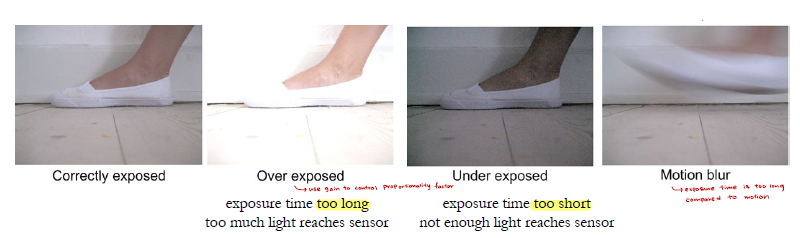
\includegraphics[width=0.7\columnwidth]{exposure}
%	\end{center}
%		\item Image formation - To accurately represent real world objects, continuous projection onto imaging sensor is used, however digital image quantize the projection into pixels
%		\item Resolution - affects file size, image of $N\times M$ with bit depth of $k$ requires $M\cdot N\cdot k$ bits
%	\end{itemize}
%	\begin{center}
%		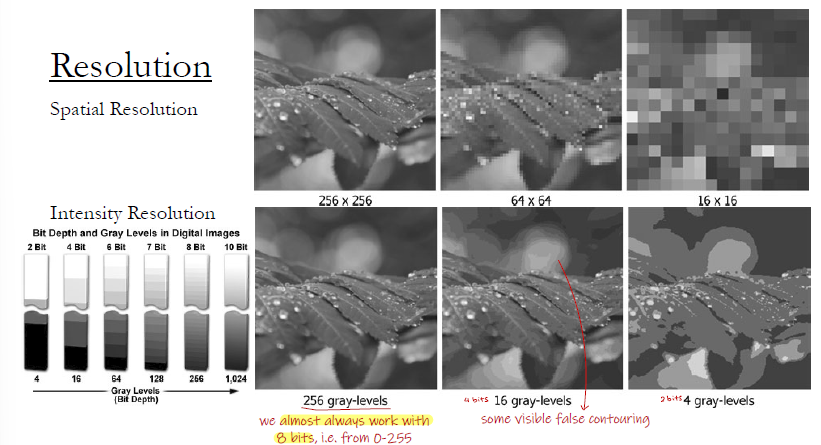
\includegraphics[width=0.7\columnwidth]{resolution}
%	\end{center}
%		\subsection{Color Capture}
%		\begin{itemize}
%			\item Typically done using a bayer filter which are 3 filters that only allow R, G and B light to pass through respectively
%			\item Bayer filters have more greens 
%		\end{itemize}
	\subsection{Colors}
	\subsubsection{Converting RGB to Grayscale}
	\begin{itemize}
		\item Grayscale Intensity = $W_R\cdot R + W_G\cdot G + W_B\cdot B$, $W_R+W_G+W_B=1$
%		\item Weights are 1/3 by default but it is also quite typical to use $W_R=0.99,W_G=0.587,W_B=0.114$ that is a good compromise for visualization purpose
	\end{itemize}
	\subsubsection{Normalized RGB}
	\begin{itemize}
		\item $(r,g,b)=\left(\frac{R}{R+G+B},\frac{G}{R+G+B},\frac{B}{R+G+B}\right)$
		\item Sometimes represented as $(r,g,I)$, $I=\frac{R+G+B}{3}$ - Intensity more informative
	\end{itemize}
	\subsection{HSV Color Space}
	\begin{itemize}
		\item \textbf{Hue}: “pure” colour (0 to 360)
		\item \textbf{Saturation}: “purity”, mixing pure colour (1) with white light (0)
		\item \textbf{Value}: achromatic mixing from 3 Color Images black (0) to white (255)
	\end{itemize}
%	\subsection{Uses of Colors}
%	\begin{itemize}
%		\item \textbf{Indexing and retrieval} through the use of color histograms - stable object representation of multicolored objects
%		\item \textbf{Color-Based Segmentation} - most common example is using green screen to segment foreground object from background
%	\end{itemize}
	\section{Point Processing and Filtering}
	\subsection{Point Processing}
	\subsubsection{Brightness}
	\begin{itemize}
		\item $x_{i,j}=p_{i,j}+b$ - image clips at 0 and 255
	\end{itemize}
	\subsubsection{Intensity Scaling}
	\begin{itemize}
		\item $x_{i,j}=a\cdot p_{i,j}$
	\end{itemize}
	\subsubsection{Image Normalization (Whitening)}
	\begin{descitemize}
		\item Removes contrast and constant additive luminance variations
		\item Mean $\mu=\dfrac{\sum_{i=1}^{I}\sum^{J}_{j=1}p_{ij}}{IJ}$
		\item Var $\sigma^2=\dfrac{\sum_{i=1}^{I}\sum^{J}_{j=1}(p_{ij}-\mu)^2}{IJ}$
		\item  $x_{ij}=\dfrac{p_{ij}-\mu}{\sigma}$
%		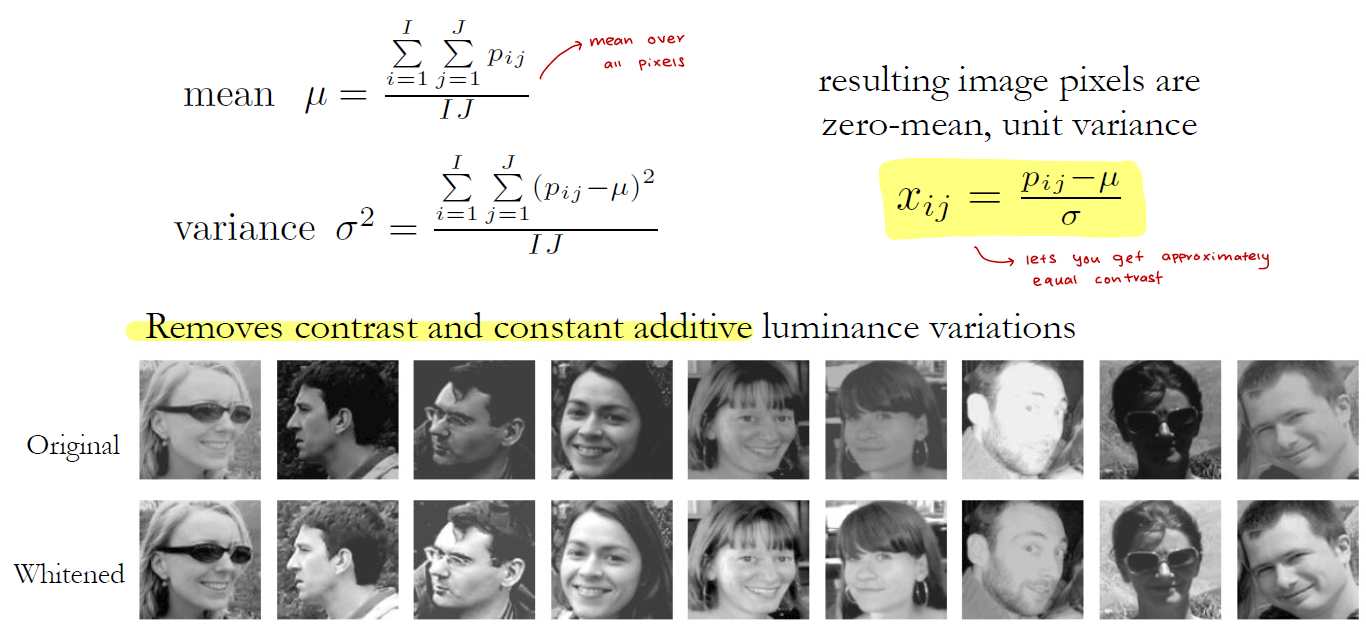
\includegraphics[width=0.7\columnwidth]{whitening}
	\end{descitemize}
	\subsubsection{Gamma Mapping}
	e.g. $x_{i,j}=255\cdot(\frac{p_{i,j}}{255})^\gamma$, non-linear transformation
%	\begin{center}
%		\includegraphics[width=0.7\columnwidth]{gamma_map}
%	\end{center}
	\subsubsection{Histogram Stretching and Equalization}
	\begin{itemize}
		\item Histogram stretching: $x = (p-f_1)\times(255/(f_2-f_1))$, $p$ is the original value, $f_1,f_2$ is the min/max value of original 
		\item Histogram Equalization: $x_{i,j} = \text{max intensity}\times\text{CDF}_{i,j}$
	\end{itemize}
%	\begin{tabular}{c c}
%		\includegraphics[width=0.5\linewidth]{hist_stretch}
%		\includegraphics[width=0.5\linewidth]{hist_equalization}
%	\end{tabular}
	\subsubsection{Uses of Histograms}
	\begin{itemize}
		\item Segmentation/Thresholding - separating foreground object from background 
		\begin{itemize}
			\item Ideally want the histogram to be bimodal but is highly unlikely in the real world
			\item Can achieve automated thresholding using Otsu's Method
			\item $T*=\arg\min w_1(T)\cdot\sigma_1^2(T)+w_2(T)\cdot\sigma_2^2(T)$\\ $\sigma_1^2(T), \sigma_2^2(T)$ - variance of pixels $\leq$ or > threshold\\
			$w_1(T),w_2(T)$ - number of pixels $\leq$ or > threshold
		\end{itemize}
		
	\end{itemize}
%	\begin{center}
%		\includegraphics[width=0.7\columnwidth]{otsu}
%	\end{center}
	\subsection{Filters}
	\subsubsection{Noises}
%	\begin{minipage}{0.3\columnwidth}
%		\begin{center}
%			\includegraphics[width=1\columnwidth]{noise}
%		\end{center}
%	\end{minipage}
%	\begin{minipage}{0.5\columnwidth}
	Can try to reduce noise using the following methods:
	\begin{itemize}
		\item replacing pixel values with average of neighbors' value
		\item Weighted Moving Average - give more weight to center pixel
		\item Gaussian Filter - blurs as well as removes Gaussian noise
		\item Median Filter - removes spikes (salt and pepper noise) with no new pixel values introduced, may lose edges
		\begin{itemize}
			\item Strategy is to take all pixel value in a 3x3 grid, sort the values and then take the value of the median
		\end{itemize}
	\end{itemize}
%	\end{minipage}
	\subsubsection{Gaussian Filter}
	\begin{itemize}
		\item $f_{uv}=\dfrac{1}{2\pi\sigma^2}e^{-\dfrac{u^2+v^2}{2\sigma^2}}$, where $\sigma$ is the scale of gaussian
		\item Sigma of Gaussian Filters affect the blurring effect more than the size of the kernel
	\end{itemize}
	\subsubsection{Sharpening Kernel}
%	\[
%	\begin{bmatrix}
%		0 & 0 & 0 \\
%		0 & 2 & 0\\
%		0 & 0 & 0
%	\end{bmatrix}
%	- \frac{1}{9}
%	\begin{bmatrix}
%		1 & 1 & 1\\
%		1 & 1 & 1 \\
%		1 & 1 & 1
%	\end{bmatrix}
%	= -\frac{1}{9}
%	\begin{bmatrix}
%		1 & 1 & 1 \\
%		1 & -17 & 1 \\
%		1 & 1 & 1
%	\end{bmatrix}
%	\]
	\begin{itemize}
		\item -1/9[[1,1,1], [1,-17,1], [1,1,1]]
		\item Combines a kernel to increase intensity of middle pixel while simultaneously applying a box filter
		\item do nothing for flat areas but stresses intensity peaks and differences with respect to the surroundings (\textbf{edges and noise is emphasized})
	\end{itemize}
	\subsubsection{Cross Correlation}
%	\begin{center}
%		\includegraphics[width=0.7\columnwidth]{cross_correlation}
%	\end{center}
	\begin{itemize}
		\item Typically want some strategies to create a padding for images - zero pad, wrap around, copy edge or reflect across edge
		\item For a kernel with width 2k+1, we need to pad by k pixels
	\end{itemize}
	\subsection{Template Matching}
	\begin{itemize}
		\item Use what you looking for as a kernel and do cross correlation on the image - any parts of the image that "matches" the template will show up as a local maxima
		\item Problem arises if there are areas where it is primarily white (gives false positive) - solution is to use normalized cross correlation
		\[x_{ij}=\dfrac{1}{|F||w_{ij}|}\sum^k_{u=-k}\sum_{v=-k}^{k}f_{uv}\cdot p_{i+u,j+v}\]
		* |$\circ$| = root of sum of squares of all elements, F is the template, $w$ is the window
		\item Normalized version scales with respect to both filter and corresponding input window
		\item Template matching is \textbf{typically inadequate} for three-dimensional scene analysis due to occlusion, changes in viewing angle and articulation of parts
	\end{itemize}
	\subsection{Convolution}
	\begin{itemize}
		\item To perform convolution, first flip the \textbf{kernel} in both direction (up-down, left-right) and apply cross correlation
		\item Has the same properties as multiplication - commutative, associative, distributes over addition, scalar factors out, identity
		\item Is \textbf{shift invariant} - output depends only on the pattern and not position of neighbors
	\end{itemize}
	\section{Gradients and Edges}
	\subsection{Why edges?}
	\begin{itemize}
		\item Carries lots of information like reflectance changes, textures, appearance, depth discontinuities, object boundaries, shadows etc.
		\item \textbf{Resilient to lighting and color} - useful for recognition
		\item Give shape and geometry information for 3D understanding
	\end{itemize}
	\subsection{Gradients}
	\begin{itemize}
		\item Edges are sharp discontinuities (first derivative) in intensity
		\item Gradient is a vector that points in the direction of most rapid change in intensity
		\begin{itemize}
			\item Gradient direction $\theta=\tan^-1(\frac{\delta f}{\delta y}/\frac{\delta f}{\delta x})$
			\item Edge strength $||\nabla f||=\sqrt{(\frac{\delta f}{\delta x})^2+(\frac{\delta f}{\delta y})^2}$
		\end{itemize}
	\end{itemize}
	\subsubsection{Sobel Filter}
	Horizontal Sobel Filter (gives \textbf{vertical} lines): [[1,0,-1], [2,0,-2], [1,0,-1]]\\
%	\[
%	\begin{bmatrix}
%		1 & 0 & -1\\
%		2 & 0 & -2\\
%		1 & 0 & -1
%	\end{bmatrix}
%	\]
	Vertical Sobel Filter (give \textbf{horizontal} line): [[1,2,1], [0,0,0], [-1,-2,-1]]
%	\[
%	\begin{bmatrix}
%		1 & 2 & 1\\
%		0 & 0 & 0\\
%		-1 & -2 & -1
%	\end{bmatrix}
%	\]
	\begin{minipage}{0.4\columnwidth}
		\begin{center}
			\includegraphics[width=1\columnwidth]{dog}
		\end{center}
	\end{minipage}
	\begin{minipage}{0.6\columnwidth}
		\begin{itemize}
			\item Other edge detection filters: Scharr (weigh central element more), Prewitt (simplest), Roberts (look at diagonal gradient)
			\item When looking for edges/gradients, it is \textbf{important to blur} it first as \textbf{differentiation is very sensitive to noise}
			\begin{itemize}
				\item note that there is a tradeoff as adding blur will also blur the edge
				\item to save on computation, we can convolve a derivative of gaussian (2nd derivative) with the image which requires only 1 convolution
			\end{itemize}
		\end{itemize}
	\end{minipage}
	\subsubsection{Effect of $\sigma$ on Derivatives}
	\begin{itemize}
		\item Larger $\sigma$ detects larger-scale edges (good detection) but has poor localization, smaller $\sigma$ detects finer edges (good localization) but has poor detection
	\end{itemize}
	\subsubsection{Laplace Filter}
	\begin{itemize}
		\item second derivative filter that can also be approximated with finite differences: [[0,1,0], [1-4,1], [0,1,0]] or with diagonals [[1,1,1], [1,-8,1], [1,1,1]]
	\end{itemize}

%	\[
%	\begin{bmatrix}
%		0 & 1 & 0 \\
%		1 & -4 & 1\\
%		0 & 1 & 0
%	\end{bmatrix}
%	\text{ OR with diagonals}
%	\begin{bmatrix}
%		1 & 1 & 1\\
%		1 & -8 & 1\\
%		1 & 1 & 1
%	\end{bmatrix}
%	\]
	\begin{itemize}
		\item Laplacian filter can be used to sharpen images by subtracting the filter from the image (i.e. X - Laplace)
		\item Can also be combined with Gaussian Filter and applied to images to get edges
		\begin{itemize}
			\item Laplacian of Gaussian Filtering leads to "zero-crossing" (the edge themselves are black and surrounded by 2 local maxima at either side) which is less convenient as compared to Derivative of Gaussian Filter as it can just be thresholded to get the edge
		\end{itemize}
	\end{itemize}
	\subsection{Canny Edge Detection}
	\begin{minipage}{0.6\columnwidth}
		\begin{center}
			\includegraphics[width=1\columnwidth]{non-max-suppression}
		\end{center}
	\end{minipage}
	\begin{minipage}{0.4\columnwidth}
		\begin{itemize}
			\item Aims to convert the thick regions of gradient in the a single pixel wide edge
			\item Steps involved:
			\begin{enumerate}
				\item Blur image and find gradients using derivative of Gaussian
				\item Find magnitude and orientation of gradient
				\item Non-maximum Suppression - thinning of "ridges" down to single pixel
				\item Hysteresis Thresholding - edge linking
			\end{enumerate}
		\end{itemize}
	\end{minipage}
	\subsubsection{Hysteresis Thresholding}
	\begin{itemize}
		\item Apply high and low threshold on NMS image
		\item Only include the low edges that are linked to the high edges and discard the rest
	\end{itemize}
%	\begin{tabular}{c c}
%		\includegraphics[width=0.5\linewidth]{non-max-suppression-eg}
%		\includegraphics[width=0.5\linewidth]{hysteresis-threshold}
%	\end{tabular}
	\section{Lines \& Hough Transform}
%	\subsection{Motivation}
%	\begin{itemize}
%		\item Edge detection gives us all edges (lines, curves, noise etc.)
%		\item Want something that only gives us straight lines, determine which points belong to which line and does something about missing edge points and noise
%	\end{itemize}
	\subsection{Hough Transform}
	\begin{itemize}
		\item Aims to answer the questions on \textbf{what is the line} given a number of points, \textbf{how many lines} there are and \textbf{which points belong to which lines}
		\item Uses a \textbf{voting technique}
		\begin{itemize}
			\item For each edge point, record a vote for each possible line that passes through that point
			\item Look for lines which receive many votes
		\end{itemize}
	\end{itemize}
	\subsection{Different Forms of Equations for Lines}
	\subsubsection{Slope Intercept Form}
	$y=mx+b$, 
	where $m$ is the slope and $b$ is the y-intercept
	\subsubsection{Double Intercept Form}
	$\frac{x}{a}+\frac{y}{b}=1$, 
	where $a$ is the x-intercept and $b$ is the y-intercept
	\subsubsection{Normal Form}
	$x\cos\theta+y\sin\theta=\rho$\\
	where $\theta$ is the angle between the respective axis to the normal, $\rho$ is the length of the normal\\
	$\rho^2=1/(1/a^2+1/b^2)$
	\subsection{Simple Line Fitting and Limitation}
	\begin{tabular}{c c}
		\includegraphics[width=0.5\linewidth]{simple_line_fitting}
		\includegraphics[width=0.5\linewidth]{simple_line_fitting_limitations}
	\end{tabular}
	\subsection{Hough Transform}
	\subsubsection{Image vs Parameter Space}
	\begin{itemize}
		\item In image space, $y$ and $x$ are the variables and $m$ and $b$ are the parameters. i.e. $y=mx+b$
		\item In parameter space, since we already know the $x$ and $y$ coords, they become the parameter instead and we are trying to find the $m$ and $b$ values. i.e. $y-mx=b$
	\end{itemize}
	\subsubsection{Different Transformation of Hough Transform}
	\begin{itemize}
		\item Using the Slope Intercept Form:
		\begin{itemize}
			\item A line in image space becomes a point in parameter space
			\item A point in image space becomes a line in parameter space
		\end{itemize}
		\item Using the Normal Form:
		\begin{itemize}
			\item Points in image space becomes sinusoids in parameter space
		\end{itemize}
		\item For circles:
		\begin{itemize}
			\item If \textbf{radius known}, a point becomes a circle in parameter space
			\item If \textbf{radius unknown}, a point becomes a cone in parameter space
		\end{itemize}
	\end{itemize}
%	\subsubsection{Line Detection with Hough Transform (Slope Intercept Form)}
%	\begin{enumerate}
%		\item Quantize Parameter Space $(m, b)$
%		\item Create Accumulator Array $A(m,b)$
%		\item Set $A(m,b)=0, \forall m,b$
%		\item For each image edge points $(x_i,y_i)$
%		
%		$\hspace{1em}$For each element $m$
%		
%		$\hspace{2em}$ Solve $b=x_im+y_i$
%		
%		$\hspace{2em}$Increment $A(m,b)=A(m,b)+1$
%		\item Threshold \& find local maxima in accumulator array
%	\end{enumerate}
	\subsubsection{Line Detection with Hough Transform (Normal Form)}
	\begin{itemize}
		\item Problem with the slope intercept form is that the range of accumulator is infinite ($b,m$ can take any values)
		\item Solve by using normal form since $-\pi\leq\theta\leq\pi$ and $0\leq\rho\leq\rho_{\text{max}}$
		\item 2 ways to write the same line:
		\begin{itemize}
			\item Positive rho: $x\cos\theta+y\sin\theta=\rho$
			\item Negative rho: $x\cos(\theta+\pi) + y\sin(\theta+\pi)=-\rho$ 
		\end{itemize}
	\end{itemize}
	\subsubsection{Hough Transform Algorithm}
	\begin{enumerate}
		\item Quantize Parameter Space $(\theta, \rho)$
		\item Create Accumulator Array $A(\theta, \rho)$
		\item Set $A(\theta, \rho)=0, \forall \theta, \rho$
		\item For each image edge points $(x_i,y_i)$
		
		$\hspace{1em}$For each element $\theta$
		
		$\hspace{2em}$ Solve $\rho=x_i\cos\theta+y_i\sin\theta$
		
		$\hspace{2em}$Increment $A(\theta, \rho)=A(\theta, \rho)+1$
		\item Threshold \& find local maxima in accumulator array
	\end{enumerate}
	Idea of hough is that each point in image space is transformed into a line in Hough Space. To see whether points lie on the same line, we just have to \textbf{find areas where the lines intersect}
	\subsubsection{Hough Transform and Noise}
	\begin{itemize}
		\item Ideally, all the lines will intersect at a point but even with noise, it is still rather easy to discern peaks 
	\end{itemize}
	\subsection{Parameterizing a Circle}
	\begin{itemize}
		\item $(x-a)^2+(y-b)^2=r^2$
		\item If we are using fixed radius, then we can only detect objects of that specific radius (e.g. If $r$ is radius of pennies then can only detect pennies)
		\item \textbf{Robust to occlusions}
	\end{itemize}
	\begin{minipage}{0.55\columnwidth}
		\begin{center}
			\includegraphics[width=1\columnwidth]{gradient_hough_circle}
		\end{center}
	\end{minipage}
	\begin{minipage}{0.45\columnwidth}
		\begin{itemize}
			\item By using gradient information, we are able to reduce the search space from a circle to a line
			\item 2 points will be $a=x-r\cos\phi, b=y-r\sin\phi$ and $a=x+r\cos\phi, b=y+r\sin\phi$ 
		\end{itemize}
	\end{minipage}
	\subsection{Generalized Hough Transform}
	\begin{tabular}{c c}
		\includegraphics[width=0.5\linewidth]{generalized_hough}
		\includegraphics[width=0.5\linewidth]{generalized_hough2}
	\end{tabular}
	\begin{itemize}
		\item To account for orientation and scale changes, we index by matched local patterns instead (visual codewords)
	\end{itemize}
	\subsection{How to do Voting process}
	\begin{itemize}
		\item Run canny on image first to minimize irrelevant tokens
		\item Choose bin size of accumulator array wisely
		\begin{itemize}
			\item Too coarse and it would cause different lines to be merged, Too fine and it will miss lines due to noise
		\end{itemize}
		\item Do "soft voting" for neighbors: $(\theta,\rho)=0.25*(\theta,\rho-1), 0.5*(\theta\rho), 0.25*(\theta,\rho+1)$
		\item Limit voting from each token (use direction of edge to reduce votes cast)
	\end{itemize}
	\subsection{Pros and Cons of Hough Transform}
	\underline{Pros}
	\begin{itemize}
		\item All points are processed independently, so can cope with occlusion, gaps
		\item Some robustness to noise: noise points unlikely to contribute consistently
		\item Can detect multiple instances of a model in a single pass
	\end{itemize}
	\underline{Cons}
	\begin{itemize}
		\item Search time complexity increases exponentially with the \# of model parameters
		\item Non-target shapes can produce spurious peaks in parameter space
		\item Quantization: can be tricky to pick a good grid size
	\end{itemize}
	\section{Image Segmentation}
	Want to separate image into coherent regions for efficiency of further processing. Segmentation make use of \textbf{clustering} but faces 2 key challenges:
	\begin{itemize}
		\item What makes 2 points similar/different - want to represent pixel with \textbf{features} (e.g. color using sum of squared difference) and compare using features
		\item How to compute overall grouping from pairwise similarities
		\begin{itemize}
			\item \textbf{K-Means}: iteratively re-assign points to the nearest cluster center
			\item \textbf{Mean-shift} clustering: estimate modes of a probability density function
		\end{itemize}
	\end{itemize}
	\subsection{k-Means Clustering}
	\begin{itemize}
		\item Choose $k$ centers as representative and label every pixel based on nearest centers (based on squared different between points and the cluster centers)
		\item Faces a "chicken and egg" problem where if we know the centers then we can allocate pixels to groups and if we knew group membership we can get center by averaging
	\end{itemize}
	\underline{Algorithm}
	\begin{enumerate}
		\item Given $K$, randomly initialize the cluster centers, $c_1,\cdots,c_k$
		\item Given cluster centers, determine points in each cluster - for each $p_i$ find closest $c_j$ and assign it to that cluster
		\item Given points in each cluster, solve for $c_j$ by taking mean of points in cluster $j$
		\item If $c_j$ > threshold, repeat 2 and 3
	\end{enumerate}
	\subsubsection{Math of K-means}
	\begin{itemize}
		\item In each iteration, we are minimizing an objective function of $\min_{c,y}\sum_{i}||p_i-c_{y_i}||^2$ (assigning points to nearest center and re-estimating center from taking mean of cluster)
		\item Eventually converges but likely to \textbf{local minimum} - gives a \textbf{non-uniform} quantization of image intensities
	\end{itemize}
	\subsubsection{Feature Selection}
	\begin{itemize}
		\item \textbf{Intensity} similarities - don't have to be spatially coherent
		\item \textbf{Color} Similarity
		\item \textbf{Intensity + Position} similarity - same colors in 2 different regions considered 2 segments
	\end{itemize}
	\subsubsection{Pros \& Cons}
	\underline{Pros}
	\begin{itemize}
		\item Simple, fast to compute
		\item Converges to local minimum of within-cluster squared error
	\end{itemize}
	\underline{Cons}
	\begin{itemize}
		\item How to set $k$?
		\item Sensitive to initial centers and outliers
		\item Detects spherical clusters
		\item Assumes means can be computed efficiently and are meaningful
	\end{itemize}
	\subsection{Superpixeling}
	Superpixels are a group of pixels that share common characteristics, e.g. pixel intensity. They ar used as inputs to other CV algos since it is a convenient and compact representation.
	\subsubsection{Distance measures}
	\begin{itemize}
		\item Color distance: $\sqrt{(r_j-r_i)^2+(g_j+g_i)^2+(b_j-b_i)^2}$
		\item Spatial distance: $\sqrt{(x_j-x_i)^2+(y_j-y_i)^2}$
		\item Composite distance: $\sqrt{d_c^2+(d_s/s)^2c^2}$, where $s = $ (\# of total pixels / \# superpixels)$^{1/2}$ 
	\end{itemize}
%	\begin{center}
%		\includegraphics[width=0.7\columnwidth]{superpixel}
%	\end{center}
	\subsection{SLIC Superpixeling Algorithm (Modified k-means)}
	\begin{enumerate}
		\item Initialize cluster center on a grid and compute initial superpixel cluster center by moving it to the \textbf{lowest gradient position} (for efficiency) in 3x3 neighborhood
		\item Assign sample by calculating distance between pixel and closest cluster center
		\item Update cluster sample
		\item Test for convergence (< Threshold)
		\item Post-process - take mean of each superpixel (Optional)
	\end{enumerate}
	\subsection{Mean-Shift Clustering}
	\begin{minipage}{0.6\columnwidth}
		\begin{center}
			\includegraphics[width=1\columnwidth]{mean-shift}
		\end{center}
	\end{minipage}
	\begin{minipage}{0.4\columnwidth}
		\begin{itemize}
			\item Mean shift is heavily influenced by $h$ which is the radius of the kernel - \textcolor{red}{decrease in $h$ will increase \# of segments}
			\item Selecting $h$ is by trial and error
		\end{itemize}
	\end{minipage}
	\subsubsection{Mean Shift Pros and Cons}
	\underline{Pros}
	\begin{itemize}
		\item General method of mode-finding
		\item No prior assumptions on cluster shape
		\item Only 1 parameter ($h$) which has a physical meaning
		\item Finds variable number of modes
		\item Robust to outliers
	\end{itemize}
	\underline{Cons}
	\begin{itemize}
		\item Output depends on $h$ and selecting $h$ is non-trivial
		\item Computationally expensive and slow to run
		\item Scales poorly with feature space dimension
	\end{itemize}
	\subsubsection{Speedups}
	\begin{itemize}
		\item No need to loop through every point - assume all points in a certain radius $r$ will belong to same cluster
		\item Assign all points within radius $c$ of search path to mode.
	\end{itemize}
	\section{Textures}
	\begin{itemize}
		\item When we want to find image boundaries, since edges $\neq$ perceived boundaries, we must rely on textures to associate with physical attribute 
		\item Textures is defined as a \textbf{pattern with repeating elements}
		\item Often, the \textbf{same thing can be an object or a texture}, depending on the scale of consideration. (e.g. a singular leaf vs a whole tree of leaves)
	\end{itemize}
	\subsection{Why Analyze Visual Textures}
	\begin{itemize}
		\item \textbf{Visual perception}: Indicative of material properties and appearance cues (shapes, boundaries, textures)
		\item \textbf{Computer Vision}: want a feature one step above basic building block of colour, simple filters, and or edges
	\end{itemize}
	\subsection{How to represent Textures?}
	\begin{minipage}{0.65\columnwidth}
		\begin{center}
			\includegraphics[width=1\columnwidth]{texture-eg}
		\end{center}
	\end{minipage}
	\begin{minipage}{0.35\columnwidth}
		\begin{itemize}
			\item One way is to use the DoG kernel and apply it to the image, calculate the mean d/dx and d/dy values (using x and y kernel of DoG) of each window and plot it
			\item Sensitive to window size - too large window will cause signal to be washed out
			\item Window size is chosen by \textbf{scale selection} (trial and error) by looking for window scale where statistic (texture representation) does not change much
		\end{itemize}
	\end{minipage}
	\subsection{Generalizing to $d$ filters}
	\begin{itemize}
		\item If we apply 2 filters, we get a 2-dimensional feature vector
		\item By applying $d$ filter, we will have $d$-dimensional feature vectors - still using euclidean distance to compare "nearness"
		\item To ensure that we can have a fair comparison between feature points, we can \textbf{normalize} them so that scaling does not matter 
	\end{itemize}
	\subsection{Gabor Filter Banks}
	\begin{center}
		\includegraphics[width=0.7\columnwidth]{filter-bank}
	\end{center}
	\begin{itemize}
		\item Typically, a combination of different patterns at various scales and orientations are in a filter bank and each of them are applied to an image to get a $n$ dimensional feature vector
		\item A easy way to generate the filters is using Gabor Filters
	\end{itemize}
	\begin{center}
		\includegraphics[width=0.5\columnwidth]{gabor-1d}
	\end{center}
%	\begin{tabular}{c c}
%		\includegraphics[width=0.5\linewidth]{gabor-1d}
%		\includegraphics[width=0.5\linewidth]{gabor-2d}
%	\end{tabular}
	\begin{itemize}
		\item Gabor 2d:  $f_{mn}=\frac{1}{2\pi\sigma^2}\exp\left[-\frac{m^2+n^2}{2\sigma^2}\right]\sin\left[\frac{2\pi(\cos[\omega]m+\sin[\omega]n)}{\lambda}+\phi\right]$
		, where m, n – coordinates of the kernel (m = n, is circular, otherwise, ellipse), $\sigma$ - rate of decay, $\omega$ - orientation of sinusoid, $\lambda$ - wavelength of sinusoid, $\phi$ - phase of sinusoid
		\item If scale is small compared to the frequency, the Gabor filters $\approx$ derivative operators
	\end{itemize}
	\subsection{Textons}
	\begin{itemize}
		\item Characterize texture by replacing each pixel with integer representing
		texture ‘type’.
	\end{itemize}
	\begin{center}
		\includegraphics[width=0.7\columnwidth]{compute-textons}
	\end{center}
	\subsubsection{Texton Histograms for Classification}
	\begin{minipage}{0.6\columnwidth}
		\begin{center}
			\includegraphics[width=1\columnwidth]{texton-histogram}
		\end{center}
	\end{minipage}
	\begin{minipage}{0.4\columnwidth}
		\begin{itemize}
			\item Each pixel represented with an ID from a texton dictionary.
			\item Texture is defined by the spatial arrangement of texton IDs, i.e. first order statistic of texton dist
			\item For a given region, compute a histogram of textons as the representation: vector storing number of occurrences of each texton
			\item Histogramming helps \textbf{reduce the effects of noise} - assumes that similar textures would have similar histograms as a whole
		\end{itemize}
	\end{minipage}
	\subsubsection{Texton Histograms for Segmentation}
	\begin{itemize}
		\item Another use for textons histograms is for segmentation - similar textures having similar histograms are clustered together
	\end{itemize}
	\subsubsection{Using Textures to Identify Boundaries}
	\begin{itemize}
		\item To identify texture boundaries at each location in a scene, we consider a disc, split into two halves by a diameter of a particular orientation. Measure the difference in texture between the two halves by comparing texton histograms and \textbf{try all possible orientation}
		\item \textbf{high distance} between histograms, suggests \textbf{more likely boundaries}
	\end{itemize}
	\section{Keypoints \& Matching}
	\subsection{General Overview - How to combine 2 images}
	\begin{enumerate}
		\item Match parts which are the same on both images - Interest point detection, feature descriptors computation, feature matching
		\item Align images based on matches (Homography)
	\end{enumerate}
	\subsection{Characteristics of Good Local Features}
	\begin{itemize}
		\item \textbf{Repeatable interest points} - (at least some of) same points found in several images despite geometric and photometric transformations (e.g. rotation, scaling, exposure diff)
		\item \textbf{Distinct descriptors} - recognizably different info that allows it to be distinguished
		\item \textbf{Efficient} - number of features << number of pixels; compact
		\item \textbf{Local} - feature occupies a relatively small area of image (robust to clutter and occlusion)
	\end{itemize}
	\subsubsection{How to look for features}
%	\begin{minipage}{0.55\columnwidth}
%		\begin{center}
%			\includegraphics[width=1\columnwidth]{feature-detect}
%		\end{center}
%	\end{minipage}
%	\begin{minipage}{0.4\columnwidth}
	\begin{itemize}
		\item Want to find regions of image where shifting the window in any direction causes a big change (aka corners)
	\end{itemize}
%	\end{minipage}
	\subsection{Corner Detection}
	\begin{itemize}
		\item To detect a corner, we first define a window ($W$) and shift the window by an offset
		\item Compare each pixel before and after by summing up the squared differences (SSD) - $E(u,v)=\sum_{(x,y)\in W}[I(x+u,y+v)-I(x,y)]^2$
		\item If SSD is high then we can consider it a corner - \textbf{extremely inefficient} to search for high SSD this way - $O(w*h*m^2*m^2)$, where $m$ is window size
	\end{itemize}
	\subsubsection{More efficient way of finding corners}
	\begin{itemize}
		\item SSD Error $E(u,v) = [u, v]\cdot[[A, B], [B, C]]\cdot[[u], [v]]$
		\item $A$ = $\sum_{(x,y)\in W}I_x^2$, $B=\sum I_xI_y$, $C=\sum I_y^2$, $I_x,I_y$ - horizontal and vertical gradients
	\end{itemize}
%	\begin{tabular}{c c}
%		\includegraphics[width=0.42\linewidth]{second-moment1}
%		\includegraphics[width=0.58\linewidth]{second-moment2}
%	\end{tabular}
	\begin{tabular}{c c}
		\includegraphics[width=0.5\linewidth]{visualize-h}
		\includegraphics[width=0.5\linewidth]{eigen-decomp}
	\end{tabular}
	\begin{tabular}{c c}
		\includegraphics[width=0.5\linewidth]{corner-math}
		\includegraphics[width=0.5\linewidth]{h-eigenvalue}
	\end{tabular}
	\begin{itemize}
		\item Special cases of $H$: 
		\begin{itemize}
			\item Horizontal edge: H = [[0, 0], [0, $C$]], Vertical edge: H = [[$A$, 0], [0 , 0]]
		\end{itemize}
	\end{itemize}
	\begin{minipage}{0.65\columnwidth}
		\begin{center}
			\includegraphics[width=1\columnwidth]{eigenvalue-to-corner}
		\end{center}
	\end{minipage}
	\begin{minipage}{0.35\columnwidth}
		\begin{itemize}
			\item We want to avoid taking min($\lambda_1, \lambda_2$) since calculating eigenvalues requires sqrt which is a computationally expensive operation
			\item Eigenvalues are always greater than 0 by definition since the H matrix is positive semi-definite
			\item Runtime: $O(w*h*m^2)$
		\end{itemize}
	\end{minipage}
	\subsection{Summary of Harris Corner Detection}
	\begin{enumerate}
		\item Compute gradient at each point in the image
		\item Compute H matrix for each image window and get their cornerness scores
		\item Find points whose surrounding window gave large corner response (R> threshold)
		\item Take the points of local maxima, i.e., perform nonmaximum suppression
	\end{enumerate}
	\subsubsection{Non-Maximum Suppression}
	\begin{itemize}
		\item \textbf{Simple} version - search for local maximas then zero-out everything else in window 
		\begin{itemize}
			\item leads to an uneven 			distribution of interest points in areas of higher contrast
		\end{itemize}
		\item \textbf{Adaptive} version - Pick corners which are both local maxima and whose response is significantly greater (e.g. 10\%) than all neighbouring local maxima within some radius $r$
	\end{itemize}
%	\subsubsection{Weighting derivative}
%	\begin{itemize}
%		\item In practice, we want to use $H=\sum_{(x,y)\in W}w_{x,y}[[I_x^2, I_xI_y], [I_xI_y, I_y^2]]$
%	\end{itemize}
	\subsection{Harris Corners Invariances}
	\begin{itemize}
		\item \textbf{Geometric} Transformation: Rotation and scaling
		\item \textbf{Photometric} Transformation: Intensity changes
		\item \textbf{Equivariance}: if we have two transformed versions of the same image, detection (locations) undergoes a similar transformation
		\item \textbf{Invariance}: image is transformed and detection (score) does not change
		\item "Detection" refers to corner location as well as probability of being detected as corner
		\item Harris corners (detected locations) are \textbf{equivariant to translation/rotation} and response (R) is \textbf{invariant to translation/rotation}
		\item Harris corner detector is \textbf{invariant to additive changes in intensity} (change in brightness) but \textbf{not invariant to scaling of intensity} (contrast)
		\begin{itemize}
			\item To find the optimal scaling, instead of computing $f$ (harris or LoG) for larger and larger window, we can implement using a fixed window size with a \textbf{gaussian pyramid} (resize image instead of changing window size)
		\end{itemize}
		\item Harris corners are \textbf{not equivariant to scaling} of image
	\end{itemize}
%	\subsection{Plot of Laplacian of Gaussian (1D)}
%	\begin{center}
%		\includegraphics[width=0.6\columnwidth]{log}
%	\end{center}
	\section{Descriptors}
	\subsection{Definition of Image Feature Descriptor}
	\begin{itemize}
		\item Descriptors are \textbf{vector representations} that mathematically characterize region in image
		\item To match images, want to measure the distance between every pair of descriptors
		\item Descriptors should be \textbf{in/equivariant} (shouldn't change under geometric/photometric transformation) and \textbf{discriminative} (unique for each point)
	\end{itemize}
	\subsection{Descriptors Variants}
	\begin{itemize}
		\item Pure intensity values - good if geometry/appearance unchanged (template matching)
		\item Image Gradients - invariant to absolute intensity values
		\item Color histogram - invariant to changes in scale and rotation
		\item Spatial histogram - some invariance to deformation but not invariant to large rotations
		\item Rotation invariant descriptors
		\begin{itemize}
			\item Harris Corner response measure - depends only on eigenvalues
			\item Local orientation - Dominant gradient direction for image patch and rotate patch according to that angle (\textbf{canonical orientation})
			\begin{itemize}
				\item To find dominant gradient, we can either average the orientations derived from gradients in region around keypoint (may overly smooth out signal and get wrong gradient direction) or use mode
			\end{itemize}
		\end{itemize}
	\end{itemize}
	\subsection{Multi-Scale Oriented Patches (MOPS)}
	\begin{itemize}
		\item 40x40 window around keypoint, subsample every 5th pixel (absorb localization error), rotate to horizontal (gives rotation invariance), normalize intensity value (robust to photometric variations), wavelet transform to 8x8 patch to get 64-dimensional descriptor
	\end{itemize}
	\subsubsection{GIST Descriptor}
	\begin{itemize}
		\item Divide image (patch) into 4x4 cell, apply Gabor Filter, compute filter response averages of each cell, size of descriptor is 4x4xN where N is size of filter bank
		\item GIST descriptor give a rough spatial distribution of the image gradients
	\end{itemize}
	\subsection{Scale Invariant Feature Transform (SIFT) Descriptors}
	\begin{itemize}
		\item Originally describes both a detector and descriptor
		\item Descriptor is invariant to scale and rotation, can handle changes in viewpoint (up to 60$^\circ$ of plane rotation), can handle significant changes in illumination, quick and efficient
	\end{itemize}
	\subsubsection{SIFT Descriptor Algorithm}
	\begin{enumerate}
		\item Take 16x16 window around detected keypoint at from image at scale matching to keypoint. Partition window into a 4x4 grid of cells (gives some sensitivity to spatial layout)
		\item Compute gradient orientations and magnitudes for each pixel; reweight magnitudes according to a Gaussian centered on keypoint and discard pixels with low magnitude
		\item Of the remaining edge orientations, create a histogram with 8 orientation bins for each cell. To be rotation invariant,
		“shift” histogram binning by the dominant orientation. Collapse into vector (16 x 8 = 128 dims).
		\item Normalize vector to unit length, clamp values based on threshold, re-normalize again for final descriptor
	\end{enumerate}
	\subsection{Feature Matching}
	\subsubsection{Feature Distance}
	\begin{itemize}
		\item Simplest approach: L2 distance (euclidean) - $||f_1-f_2||$ (sum of squared difference)
		\begin{itemize}
			\item Possibility of giving small distances for ambiguous matches
		\end{itemize}
		\item Better approach - ratio distance: $||f_1-f_2||/||f_1-f_2'||$, $f_2'$ is the 2nd best match
	\end{itemize}
	\subsubsection{Evaluating Feature Matches}
%	\begin{center}
%		\includegraphics[width=0.8\columnwidth]{evaluation}
%	\end{center}
	\begin{itemize}
%		\item True positives: \# of correct matches
%		\item False negatives: \# of incorrect matches
%		\item True negatives: keypoints that should not be matched (appears in one image but not the other)
%		\item False negatives: keypoint detected in both but not matched
%		\item Recall: $\frac{\text{\# of true positives}}{\text{\# of true positives + false negatives}}$
%		\item Specificity = $\frac{\text{\# of true negatives}}{\text{\# of true negatives + false positives}}$
		\item Precision: TP / (TP + FP), Recall: TP / (TP + FN), Specificity: TN / (TN + FP)
		\item If threshold $\uparrow$, TP and FP $\uparrow$
	\end{itemize}
	\section{Homography}
	To stitch images from different viewpoints, it is not enough to use translation only stitching. Homography is applied to \textbf{project images onto the same plane}
	\subsection{Image Projections}
	Translation, Euclidean (Rotation), Similarity (Scaling), Affine (diff x-y scaling but still parallel aka parallelogram), Projective (Homography, resulting image look like a rhombus)
%	\begin{center}
%		\includegraphics[width=0.7\columnwidth]{2d-transforms}
%	\end{center}
	\subsection{Applying a homography}
	\begin{center}
		\includegraphics[width=0.6\columnwidth]{apply-homography}
	\end{center}
	\subsection{Solving for H using DLT}
	Given ${p_i,p_i'}$ solve for H such that $P_i'=H\cdot P_i \forall i$
	\begin{enumerate}
		\item For each correspondence, create 2x9 matrix $A_i = [[-x, -y, -1, 0, 0, 0, xx', yx', x'], [0,0,0,-x,-y,-1,xy',yy',y']]$
		\item Concatenate into single $2n \times 9$ matrix $A$
		\item Compute SVD of $A=U\Sigma V^T$
		\item Store singular vector of smallest singular value $h=v_{\hat{i}}$
		\item Reshape to get $H$ (3x3 vector)
	\end{enumerate}
	\subsubsection{Drawbacks of DLT}
	\begin{itemize}
		\item DLT uses linear least squares estimation which is only applicable when actual transformation between two images is linear
		\item Sensitive to scaling in pixel space - solved by normalization (compulsory for DLT)
		\item DLT does not deal well with outliers - solved using RANSAC
	\end{itemize}
	\subsection{When are Homographies Applicable}
	\begin{itemize}
		\item Scene is planar or approximately planar (very far away or has small depth variation)
		\item scene is captured under camera rotation only
	\end{itemize}
	\subsection{RANSAC}
	\begin{itemize}
		\item DLT find average transform using L2 distance, easily corrupted by bad correspondences
		\item RANSAC aims to solve that by having \textbf{random sample consensus} for a set of noisy observations as a 2 stage process - classify inlier vs outlier, fit model to only inliers
	\end{itemize}
	\subsubsection{RANSAC Loop}
	\begin{enumerate}
		\item Randomly get (min 4) correspondence - take as little as possible to minimize chance of picking outlier (4 because H matrix has 8 degree of freedom, each point gives 2 equations)
		\item Compute H using DLT and count inliers, keep H if largest number of inliers 
	\end{enumerate}
	For best H with most inliers, recompute using all inliers
	\subsubsection{RANSAC Parameters}
	\begin{itemize}
		\item $\partial$ - distance threshold to consider as inlier (obtained using trial and error)
		\item N - number of iterations of RANSAC loop (can be solved using ratio of outlier vs inlier)
		\begin{itemize}
			\item N = $\frac{\log(1-p)}{\log(1-(1-e)^s)}$, where $e$ is the probability that a point is an outlier, $p$ is the probability that at least one set of points sampled does not contain any outliers, $s$ is the number of points we draw per iteration (2 for a line, 3 for quadratic)
		\end{itemize}
	\end{itemize}
	\subsection{Image Warping}
	\begin{itemize}
		\item Based on the homography, we can warp image into new plane, however discretization causes problems
		\begin{itemize}
			\item certain destination pixels are not covered
			\item many pixels might map to the same destination - solved by "distributing" (averaging) intensity over neighbouring pixels (splatting)
		\end{itemize}
	\end{itemize}
	\section{Optical Flow}
	\begin{itemize}
		\item Optical flow is an instantaneous velocity measurement for direction and speed of image data across visual field
		\item Key assumptions: Color constancy (allows for pixel to pixel comparison), small motion (allows for linearization of brightness constancy constraint)
	\end{itemize}
	\subsection{Brightness Constancy Equation}
	\begin{minipage}{0.55\columnwidth}
		\begin{center}
			\includegraphics[width=1\columnwidth]{brightness-constancy}
		\end{center}
	\end{minipage}
	\begin{minipage}{0.45\columnwidth}
		\begin{itemize}
			\item $\frac{dI}{dt}=\frac{\partial I}{\partial x}\frac{dx}{dt}+\frac{\partial I}{\partial y}\frac{dy}{dt}+\frac{\partial I}{\partial t}= 0$
			\item $I_xu+I_yv+I_t=0$\\ $I_x, I_y$ is the x and y gradients, $u,v$ are the flow velocities, $I_t$ is the temporal gradient
			\item $I_x, I_y$ are computed using sobel/scharr filters, $I_t$ is computed using frame $t+1-t$
			\item Currently, solving the equation will give us solutions that lie on a line (infinitely many solutions), need more constraints to limit solution space
		\end{itemize}
	\end{minipage}
	\subsection{Lucas-Kanade Flow}
	\begin{itemize}
		\item Constant flow assumption - assumes that surrounding patch in 5x5 area has same displacements which gives us 25 equations
	\end{itemize}
	\begin{center}
		\includegraphics[width=0.7\columnwidth]{lucas-kanade}
	\end{center}
	\begin{itemize}
		\item For $A^TA\hat{x} =A^Tb$ to be solvable: 
		\begin{itemize}
			\item $A^TA$ should be invertible, determinant of $A^TA$ should not be too small, $\lambda_1, \lambda_2$ should not be too small, $\lambda_1/\lambda_2$ should not be too large ($\lambda_1>>\lambda_2$)
		\end{itemize}
		\item Lucas-Kanade \textbf{works best on corners} where $\lambda_1,\lambda_2$ are big
	\end{itemize}
	\subsection{Aperture Problem}
	\begin{itemize}
		\item If a motion sensor has a finite receptive field, it makes a homogeneous contour seem locally ambiguous (we can only find out the $u$ or $v$ components)
		\item Want patches with different gradients to avoid aperture problem (aka corners)
	\end{itemize}
	\subsection{Gaussian Pyramid}
	\begin{itemize}
		\item When movements are too large (> 1px), we face a problem of aliasing where the nearest match is a wrong correspondence
		\item To fix this, we want to downsample the image to get "smaller" motions (solved using LK) and then iteratively apply this motion to the original image and upsample
		\item Ideally this brings the original image to a point where it has only a small motion relative to the next reference frame
	\end{itemize}
	\subsection{Horn-Schunk Optical Flow}
	\begin{itemize}
		\item Enforce brightness constancy - for every pixel: $\min_{u,v}[I_xu_{i,j}+I_yv_{i,j}+I_t]^2$
		\item Enforce smooth flow field - $\min_u(u_{i,j}-u_{i+1,j})^2$, patch don't share same (u,v)
		\item Key idea - $\min_{u,v}\sum_{i,j}{E_s(i,j)+\lambda E_d(i,j)}$, $E_s$ is the smoothness and $E_d$ is the brightness constancy (uses gradient descent algo)
	\end{itemize}
	\subsubsection{Horn-Schunk Algorithm}
	\begin{enumerate}
		\item Precompute image gradients $I_y, I_x$ and temporal gradient $I_t$
		\item Initialize flow field ($u=0, v=0$)
		\item While not converged $\rightarrow$ compute flow field updates\\
		$\hat{u}_{kl}=\overline{u}_{kl}-\frac{I_x\overline{u}_{kl}+I_y\overline{v}_{kl}+I_t}{\lambda^{-1}+I_x^2+I_y^2}I_x$, $\hat{v}_{kl}=\overline{v}_{kl}-\frac{I_x\overline{u}_{kl}+I_y\overline{v}_{kl}+I_t}{\lambda^{-1}+I_x^2+I_y^2}I_y$
	\end{enumerate}
	\subsection{Lucas-Kanade vs Horn-Schunk}
	\underline{Lucas-Kanade}
	\begin{itemize}
		\item feature-based method that extracts visual features and tracks them over multiple frames
		\item Generates only sparse motion fields, but is more robust at tracking
		\item Suitable when image motion is large (10s of pixels)
	\end{itemize}
	\underline{Horn-Schunk}
	\begin{itemize}
		\item Directly method that recovers image motions at every pixel based only on spatio-temporal
		image brightness variations
		\item Dense motion fields, but sensitive to appearance variations
		\item Suitable for video and when image motion is small
	\end{itemize}
%	\subsection{Warping}
%	\begin{itemize}
%		\item Mapping (transformation relating destination (x,y) for every source (u,v), e.g. homography) + Resampling (estimate arbitrary location somehow, nearest neighbor, bi-linear interpolation)
%		\item Since a flow field is a mapping of pixel from one frame to the next, the \textbf{finer the resolution the more precise the flow estimate}
%		\item 
%	\end{itemize}
	\section{Tracking}
	\subsection{Methods of finding template in image}
	\begin{itemize}
		\item Template matching - slow, combinatory, finds global solution
		\item Multi-scale template matching - scale \textbf{image} and match template, faster, local optima
		\item Local refinement based on some initial guess - fastest, local optima
	\end{itemize}
	\begin{center}
		\includegraphics[width=0.65\columnwidth]{notations}
	\end{center}
	\subsection{Lucas-Kanade Alignment}
	\begin{itemize}
		\item Warp image - $I(\mathbf{W}(x;p))$
		\item Compute error image - [$T(x)-I(\mathbf{W}(x;p))$], Compute gradient - $\triangledown I(x')$
		\item Evaluate Jacobian - $\partial{W}/{\partial p}$
		\item Compute Hessian Approximation - $H = \sum_{x}\left[\triangledown I\cdot \partial W/\partial p\right]^T\left[\triangledown I \cdot\partial W/\partial p\right]$
		\item Compute - $\Delta p=H^{-1}\sum_{x}\left[\triangledown I\cdot\partial W/\partial p\right]^T[T(x)-I(W(x;p))]$
		\item Update parameters - $p\leftarrow p + \Delta p$
	\end{itemize}
%	\begin{center}
%		\includegraphics[width=0.7\columnwidth]{lucas-kanade-alignment}
%	\end{center}
	\subsection{How to choose good features for tracking}
	\begin{itemize}
		\item Want to avoid smooth regions and edges - corners chosen as good features
	\end{itemize}
	\subsection{KLT Algorithm for Feature Tracking}
	\begin{itemize}
		\item Find corners satisfying min($\lambda_1, \lambda_2>\lambda$) for Hessian
		\item Loop over corners $\rightarrow$ compute displacement to next frame using Lucas-Kanade, store displacement and update corner positions, (optional) add more corners every M frames
		\item Return long trajectories for each corner
	\end{itemize}
	\subsection{Challenges of Feature-Based Tracking}
	\begin{itemize}
		\item Figuring out which features can be tracked
		\item Efficiency: How to track them efficiently
		\item Accuracy: Changing appearance of some points e.g. rotations, movement into shadows, drift - accumulation of small errors as appearance model updates
		\item Appearance / disappearance of points
	\end{itemize}
	\subsection{Tracking with Template Matching}
	\begin{itemize}
		\item Initialize bounding box of object to be tracked manually
		\item Compute template descriptor for target
		\item Search for similar descriptor in neighborhood of next frame - look for maxima
		\item Update target and descriptor
		\item Template-based tracking algorithm differ in the way they:
		\begin{itemize}
			\item Represent candidates: gradient features, histogramming, deep features
			\item Search for candidates: limit search space based on previous results
			\item Solve the mode-finding problem: leverage previous locations to help with local max
			\item Update target's template: update as the track progresses
		\end{itemize}
		\item Evaluation Measure: $|B_{gt}\bigcap B_p|/|B_{gt}\bigcup B_p$
	\end{itemize}
	\subsubsection{MOSSE Filter}
	\begin{tabular}{c c}
		\includegraphics[width=0.5\linewidth]{mosse1}
		\includegraphics[width=0.5\linewidth]{mosse2}
	\end{tabular}
	\subsection{Tracking Issues}
	\begin{itemize}
		\item Initialization typically done manually but background subtraction detection is also used
		\item Catastrophic errors: Occlusion and clutter, exit of frame, multiple objects
		\item Gradual errors: drifting due to accumulation of small errors over time
	\end{itemize}
	\section{Deep Learning}
	\subsection{Data-Driven Image Classification}
	Collect db of img w/ labels $\rightarrow$ use ML to train img classifier $\rightarrow$ evaluate classifier on test img
	\subsection{AI vs ML vs Deep Learning}
	\begin{itemize}
		\item \textbf{AI} - imparting cognitive abilities to machine, \textbf{ML} - algo and models to perform tasks based on patterns/inference instead of specific instructions, \textbf{DL} - branch of ML using neural nets (uses cascade of multiple layers of nonlinear processing units for feature extraction/transformation)
		\item Deep Learning = Big Data + labels + Known Algos + Computing Power (GPUs)
	\end{itemize}
	\subsection{Perceptrons}
	\begin{tabular}{c c}
		\includegraphics[width=0.6\linewidth]{perceptron}
		\includegraphics[width=0.4\linewidth]{perceptron-eg}
	\end{tabular}
	\subsection{Stationarity}
	\begin{itemize}
		\item To reduce number of parameters in a neural network, we make use of \textbf{stationarity} which states that statistics is similar at different locations (e.g. all edges will have same characteristics no matter where they are)
		\item We now take each "local" perceptron as a filter/kernel that all has the \textbf{same learned weight} $w$ and then do convolution over the entire image
		\begin{itemize}
			\item Param is \textbf{independent of img size} and is calculated by \# of filters $\times$ kernel size
		\end{itemize}
		\item Output = 0 if $w\cdot x + b \leq 0$ or 1 otherwise
		\begin{itemize}
			\item Output if using the stationarity property will be a 2d vector since each output is linked to an area in the original image
		\end{itemize}
		\item Locally Linear + Stationarity = Convolution
		\begin{itemize}
			\item extent of local connectivity determines kernel size
			\item Single filter $\rightarrow$ single feature map, multiple filters $\rightarrow$ multiple feature maps
			\item Each feature map is a channel of output
			\item \textbf{Param sharing} built in, leads to equivariant representation - output changes w/ input
		\end{itemize}
	\end{itemize}
	\subsection{Pooling}
	\begin{itemize}
		\item Pooling makes large distortions become smaller to give more invariance
		\item Max pooling: take max value in a $n\times n$ area 
	\end{itemize}
	\subsection{Convolution-pooling-convolution}
	\begin{itemize}
		\item Interleaving convolutions and pooling causes later convolutions to capture a larger fraction of the image with the same kernel size
		\item Set of image pixels that an intermediate output pixel depends on = receptive field
		\begin{itemize}
			\item assume that in a neural net layer we care about "local neighborhoods"
			\item Composition of layers will expand from local to global 
		\end{itemize}
		\item Convolutions after pooling increase the receptive field
		\item e.g. of CNN flow $\rightarrow$ Conv -> ReLU -> Conv -> ReLU -> Pool -> $\cdots$
	\end{itemize}
	\end{multicols*}
\end{document}
